%add the next in child files %!TEX root = mars-amr.tex

\documentclass{article}
\usepackage[utf8]{inputenc}
\usepackage{graphicx}
\usepackage{amsmath}
\usepackage{tikz}
\usepackage{mathptmx} 
\usepackage{listings}
\usepackage{xcolor} 
\usepackage{tikz} % To generate the plot from csv
\usepackage{pgfplots}
\pgfplotsset{compat=1.12} 
\usepackage{pgfplotstable}
\usetikzlibrary{backgrounds}
% \usepackage[percent]{overpic}

\usepackage{draftwatermark}
\SetWatermarkText{DRAFT}
\SetWatermarkScale{1}

\definecolor{avgcolor}{rgb}{0,1.,0.5}
\definecolor{maxcolor}{rgb}{1,0.5,0}
\definecolor{mincolor}{rgb}{0,0.5,1}

% % set the default code style
% \lstset{
%     frame=tb, % draw a frame at the top and bottom of the code block
%     tabsize=4, % tab space width
%     showstringspaces=false, % don't mark spaces in strings
%     numbers=left, % display line numbers on the left
%     % commentstyle=\color{green}, % comment color
%     % keywordstyle=\color{blue}, % keyword color
%     % stringstyle=\color{red} % string color
% }


\definecolor{cppred}{rgb}{0.6,0,0} % for strings
\definecolor{cppping}{rgb}{1,0.7,0.7} % for numbers
\definecolor{cppgreen}{rgb}{0.25,0.5,0.35} % comments
\definecolor{cpppurple}{rgb}{0.5,0,0.35} % keywords
\definecolor{cppdocblue}{rgb}{0.25,0.35,0.75} % cppdoc

\newcommand{\todo}[1]{{\color{cppdocblue} #1 }} 



\lstset
{
	language=C++, 
	basicstyle=\scriptsize\ttfamily,
	numberstyle=\tiny\color{cpppink},
	keywordstyle=\color{cpppurple}\bfseries,
	stringstyle=\color{cppred},
	commentstyle=\color{cppgreen},
}

\newcommand{\cppdouble}{{\color{cpppurple} double}}
\newcommand{\cppint}{{\color{cpppurple} int}}
\newcommand{\cppif}{{\color{cpppurple} if}}
\newcommand{\cppwhile}{{\color{cpppurple} while}}
\newcommand{\cppelse}{{\color{cpppurple} else}}

\title{MARS: Adaptive Simplicial Mesh Refinement}
% \author{Patrick Zulian}
\begin{document}
\maketitle

\section{Introduction}
MARS is a $N$-dimensional mesh (tested up to 6D) refinement C++ library. Currently the refinement algorithms are only available for serial run-times, but an MPI-based parallel implementation is in development.

\section{Edge bisection algorithm}
\label{sec:bisection}

The general refinement strategy implemented in this library is based on recursive edge bisection. The algorithm consists of the following steps:

\begin{enumerate}
	\item Mark elements for refinement.
	\item For each marked element select the edge to bisect.
	\item Refine the element by bisect the edge and mark the incident elements for refinement.
	\item Go back to 2 and repeat until the mesh is conforming.
\end{enumerate}

Figure~\ref{fig:two_dim} shows consecutive refinement steps on a 2D mesh, and Figure~\ref{fig:sphere} shows the final mesh for a hyper-spherical refinement pattern for both 2D and 3D meshes.

\begin{figure} \centering \footnotesize
	\parbox{0.5\linewidth}{
	
\includegraphics[width=0.32\linewidth]{figures/mesh_2_bisect_1} \hfill
	
\includegraphics[width=0.32\linewidth]{figures/mesh_2_bisect_2} \hfill
	
\includegraphics[width=0.32\linewidth]{figures/mesh_2_bisect_3} \par
	
\includegraphics[width=0.32\linewidth]{figures/mesh_2_bisect_4} \hfill
	
\includegraphics[width=0.32\linewidth]{figures/mesh_2_bisect_5} \hfill
	
\includegraphics[width=0.32\linewidth]{figures/mesh_2_bisect_6} \par
	
\includegraphics[width=0.32\linewidth]{figures/mesh_2_bisect_7} \hfill
	
\includegraphics[width=0.32\linewidth]{figures/mesh_2_bisect_8} \hfill
	
\includegraphics[width=0.32\linewidth]{figures/mesh_2_bisect_9} \par
	}
	\caption{Steps of the bisection algorithm.}
	\label{fig:two_dim}
\end{figure}

\begin{figure} \centering \footnotesize
	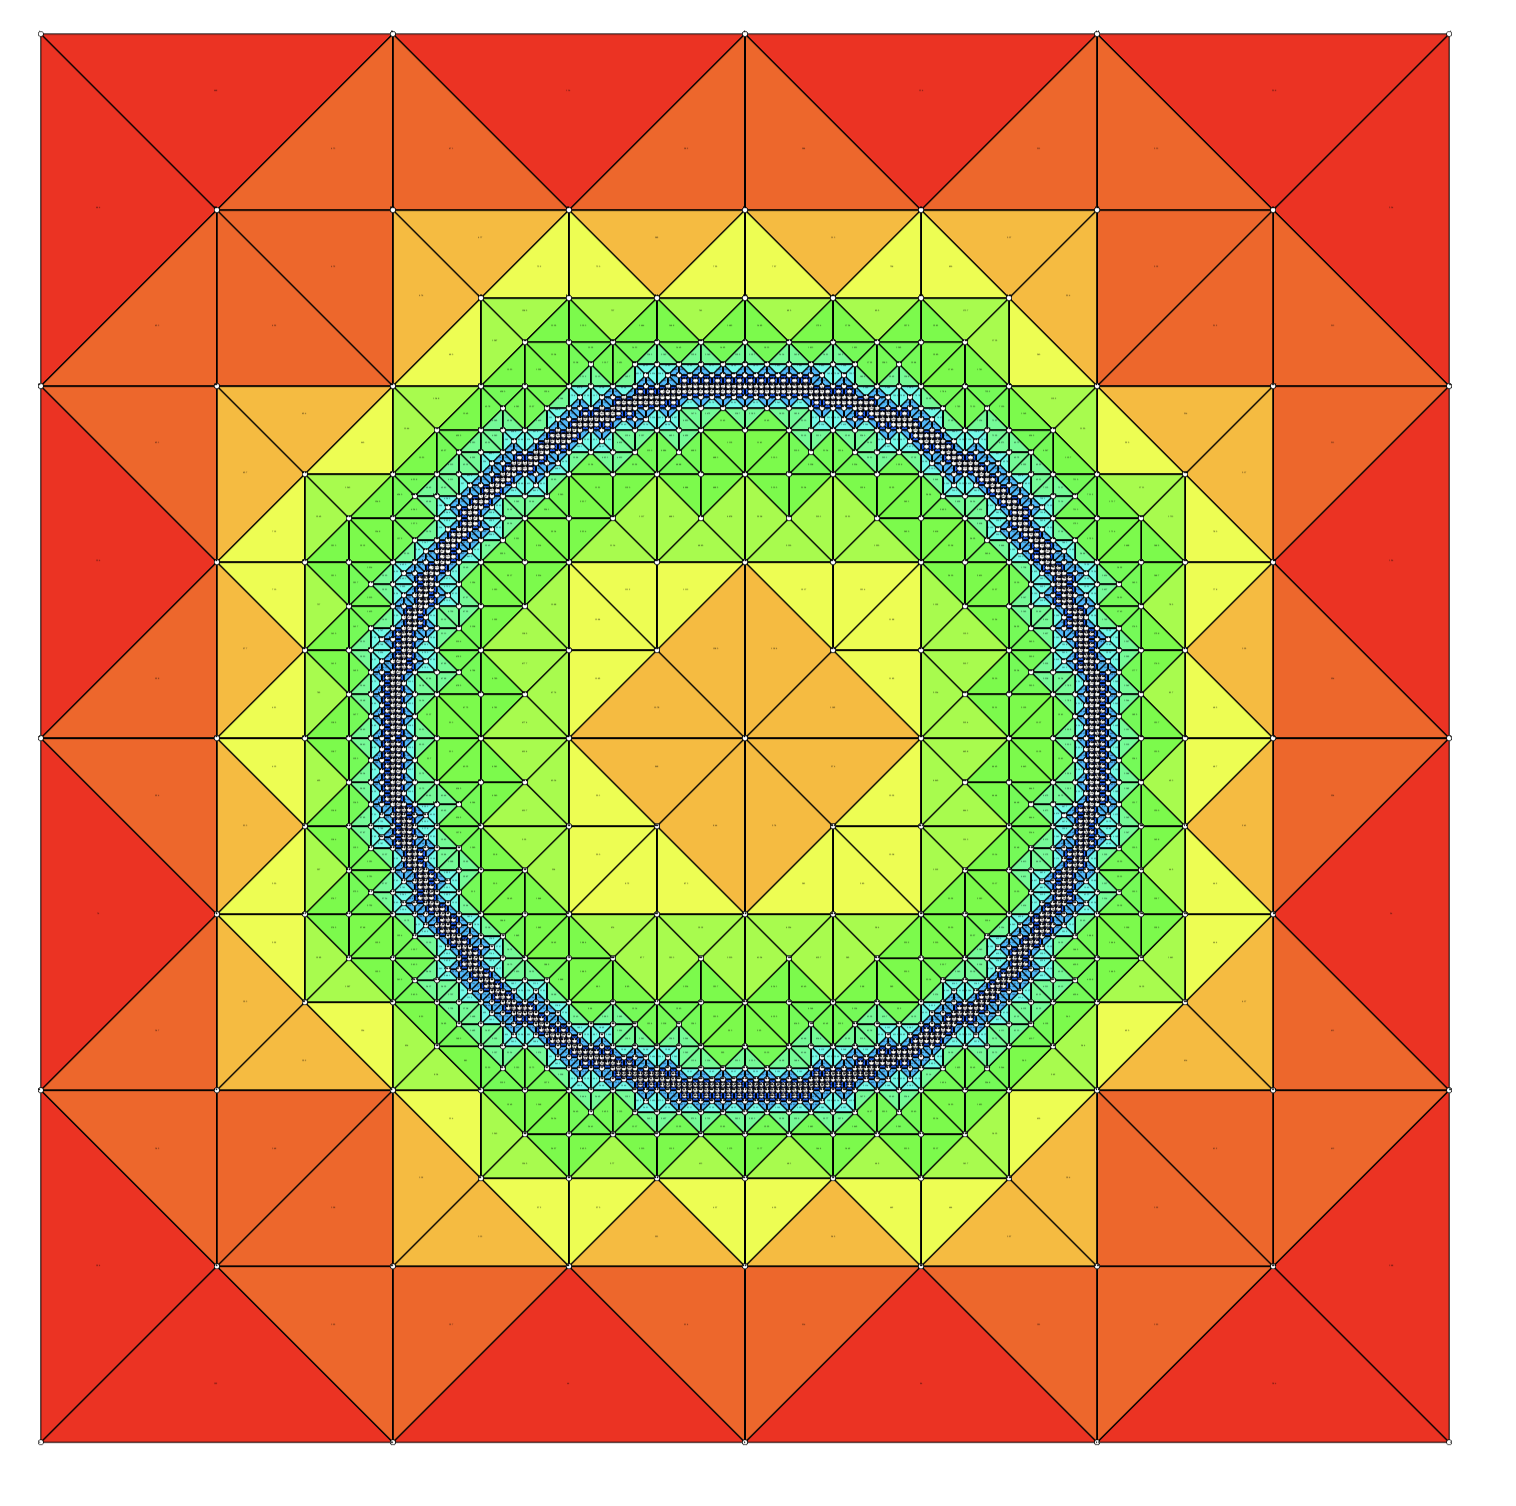
\includegraphics[width=0.40\linewidth]{figures/2d_sphere} \hfill
	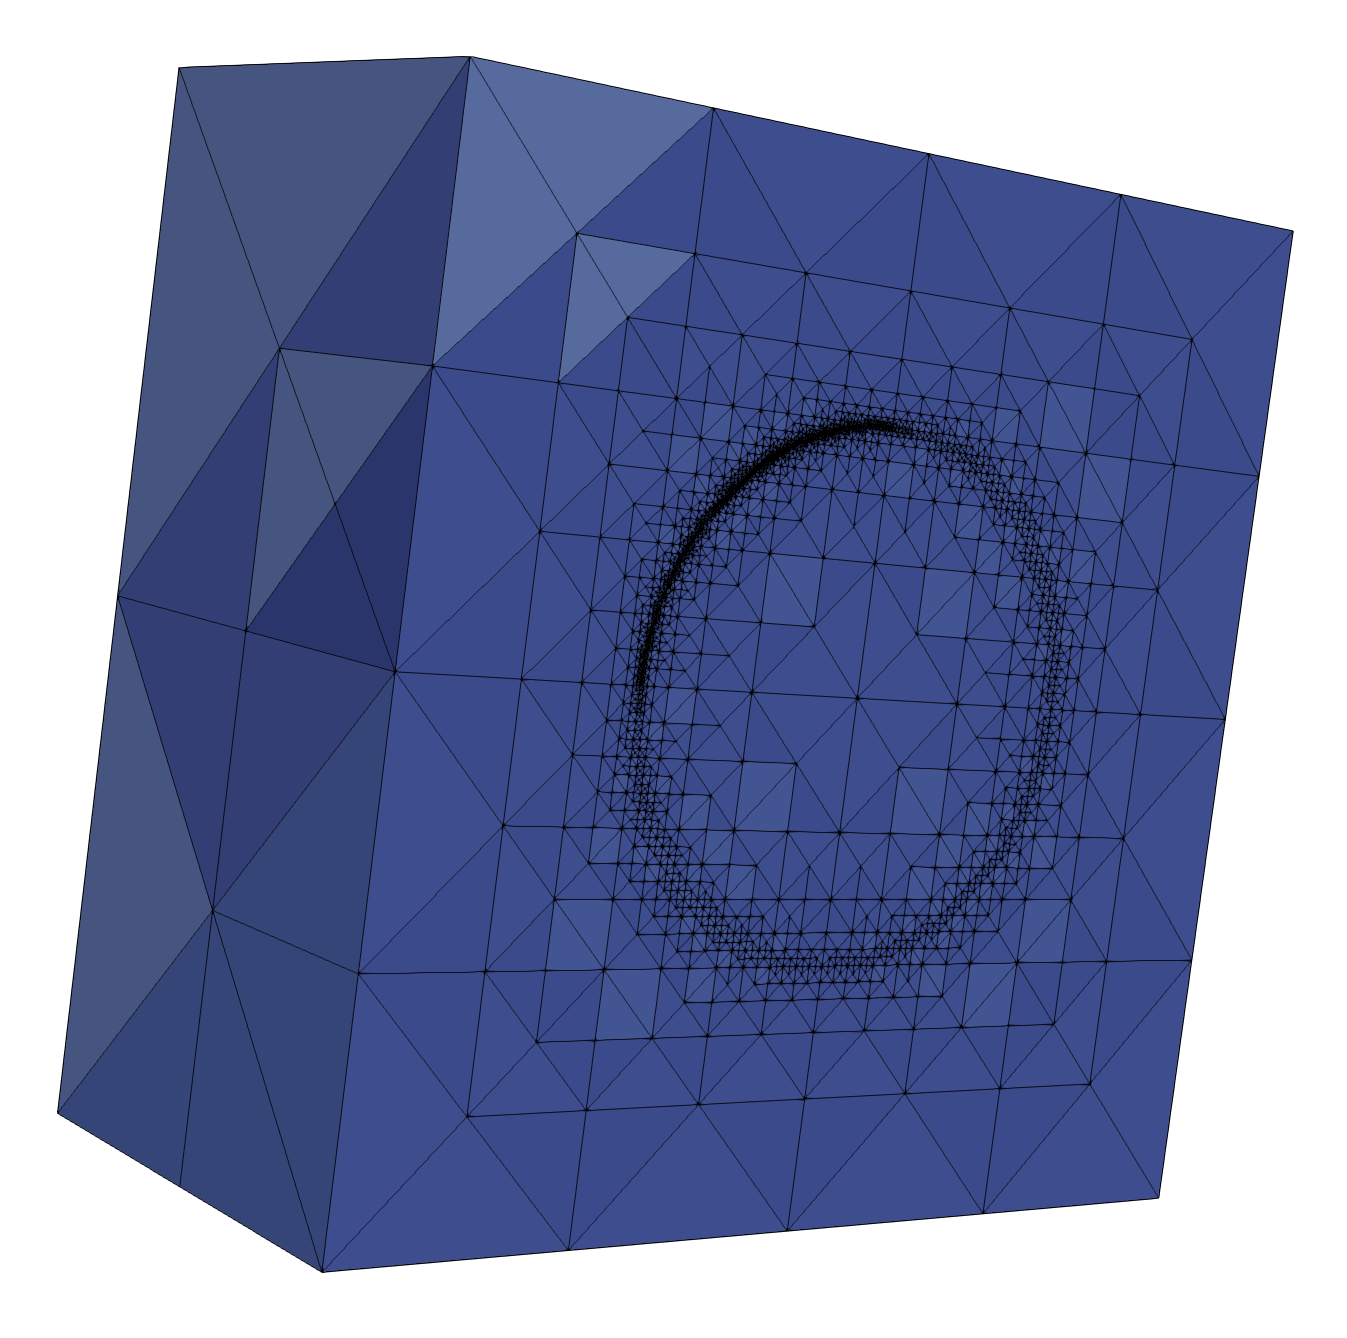
\includegraphics[width=0.40\linewidth]{figures/3d_sphere} 
	\caption{Result for sphere refinement pattern. Left: 2D. Right: 3D.}
	\label{fig:sphere}
\end{figure}

\section{Edge selection}

We have implemented the following strategies:

\begin{itemize}
	\item Recursive longest-edge bisection.
	\item Newest vertex bisection.
\end{itemize}

\section{Recursive edge selection}

When refining an element $S$ incident to an edge $e_1$ that has been selected for refinement, we first select the appropriate edge $e_2$ (which does not have to respect $e_1 = e_2$).
For the algorithm to terminate we have to finally select $e_1$ from one of the descendants of $S$.
Figure~\ref{fig:recur} shows the difference between non-recursive and recursive edge selection.

\begin{figure} \centering \footnotesize
	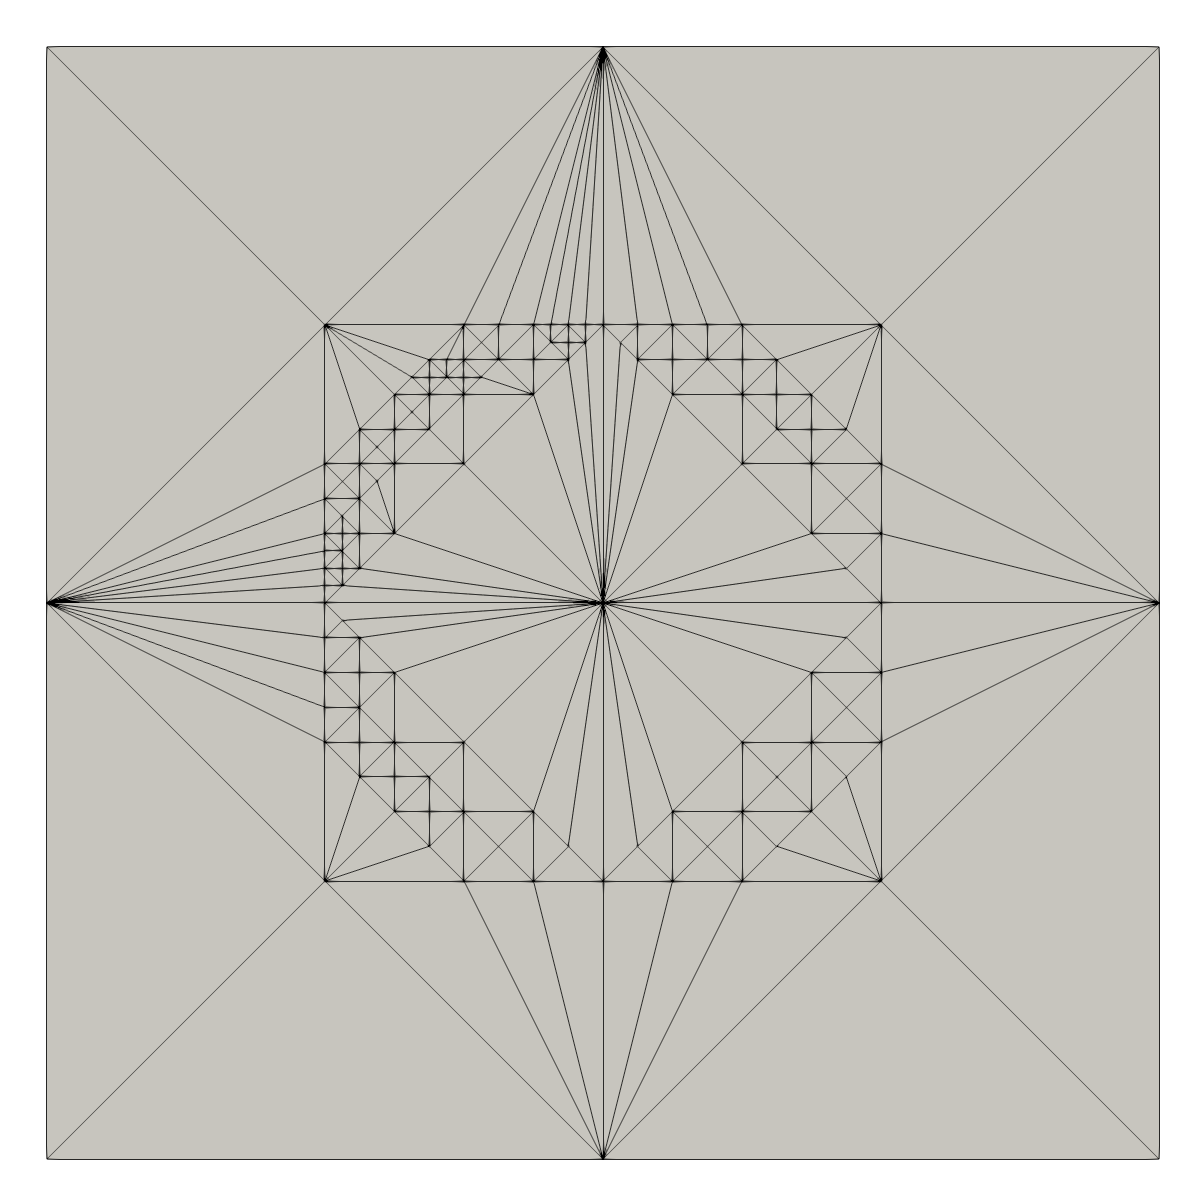
\includegraphics[width=0.45\linewidth]{figures/non-recursive} \hfill
	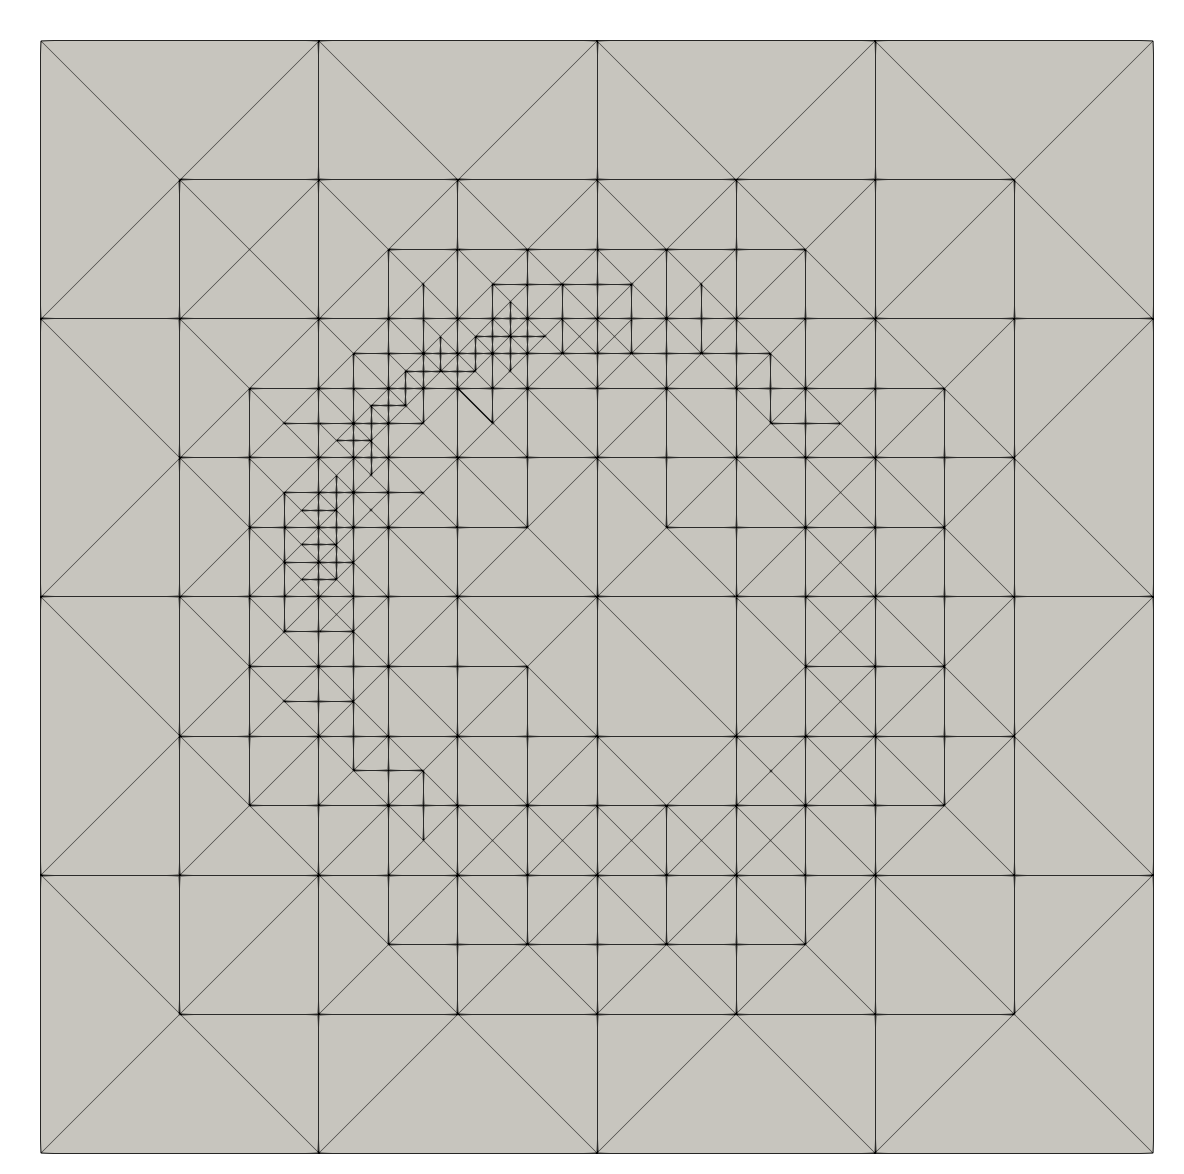
\includegraphics[width=0.45\linewidth]{figures/recursive}
	\caption{Non-recursive vs. recursive (3D).}
	\label{fig:recur}
\end{figure}



\section{Quality}

For measuring the condition of an element $S$ we use the following metrics:
\begin{align*}
	\alpha(S) &= \frac{\left( \sum_{i=1}^{D+1} \text{vol}(\text{side}_i(S))/(D+1)  \right)}{\text{vol}(S)} \\
	\tau(S) &= \frac{\max_{i=1}^{D+1} \text{vol}(\text{side}_i(S))}{\min_{i=1}^{D+1} \text{vol}(\text{side}_i(S))}
\end{align*}


Longest-edge bisection is known to generate stable and high quality refinements as shown includegraphics Figure~\ref{fig:quality2}, Figure~\ref{fig:quality3}, and Figure~\ref{fig:quality4}. 

%While the longest-edge criterion is superior, the hybrid approach (newest vertex + longest edge) stays in the same order of magnitude for the degrading element quality. With further experiments it appears that the hybrid approach does not consistently generates conforming meshes.

%!TEX root = ../mars-amr.tex

\begin{figure} \centering \footnotesize
\hfill
\begin{tikzpicture}[tight background]% , show background rectangle]
    \begin{semilogxaxis}[
        height=0.48\linewidth,
        % width=\pgfplotswidth,
        width=0.48\linewidth,
        yticklabel style={align=right,inner sep=0pt,xshift=-0.3em},
        %
        scaled ticks=false,
        legend entries={$\alpha_\text{max}$,$\alpha_\text{avg}$,$\alpha_\text{min}$},
        legend style={at={(1,0.9)},anchor=north east,fill=none,draw=none,legend cell align=left}
    ]
    %
    \addplot[
        color=maxcolor,
        mark=*,
        mark size=1pt,
    ]
    table[x=ne,y=alpha max,col sep=comma] {charts/quality2.csv}; 
    %
    \addplot[
        color=avgcolor,
        mark=*,
        mark size=1pt,
        %skip coords between index={0}{1},
    ]
    table[x=ne,y=alpha avg,col sep=comma] {charts/quality2.csv}; 
    %
    \addplot[
        color=mincolor,
        mark=*,
        mark size=1pt,
    ]
    table[x=ne,y=alpha min,col sep=comma] {charts/quality2.csv}; 

    \end{semilogxaxis}
\end{tikzpicture} \hfill
%
\begin{tikzpicture}[tight background]% , show background rectangle]
    \begin{semilogxaxis}[
        height=0.48\linewidth,
        % width=\pgfplotswidth,
        width=0.48\linewidth,
        yticklabel style={align=right,inner sep=0pt,xshift=-0.3em},
        %
        scaled ticks=false,
        legend entries={$\tau_\text{max}$,$\tau_\text{avg}$,$\tau_\text{min}$},
        legend style={at={(1,0.9)},anchor=north east,fill=none,draw=none,legend cell align=left}
    ]
    %
    \addplot[
        color=maxcolor,
        mark=*,
        mark size=1pt,
    ]
    table[x=ne,y=tau max,col sep=comma] {charts/quality2.csv}; 
    %
    \addplot[
        color=avgcolor,
        mark=*,
        mark size=1pt,
        %skip coords between index={0}{1},
    ]
    table[x=ne,y=tau avg,col sep=comma] {charts/quality2.csv}; 
    %
    \addplot[
        color=mincolor,
        mark=*,
        mark size=1pt,
    ]
    table[x=ne,y=tau min,col sep=comma] {charts/quality2.csv}; 

    \end{semilogxaxis}
\end{tikzpicture} \hfill
%
\caption{Quality of recursive longest edge refinement (lower is better). The $x$-axis represents the number of elements in the mesh (2D), and the $y$-axis the quality metric.
Left $\alpha$, Right $\tau$.}
\label{fig:quality2}
\end{figure}

%!TEX root = ../mars-amr.tex

\begin{figure} \centering \footnotesize
\hfill
\begin{tikzpicture}[tight background]% , show background rectangle]
    \begin{semilogxaxis}[
        height=0.48\linewidth,
        % width=\pgfplotswidth,
        width=0.48\linewidth,
        yticklabel style={align=right,inner sep=0pt,xshift=-0.3em},
        %
        scaled ticks=false,
        legend entries={$\alpha_\text{max}$,$\alpha_\text{avg}$,$\alpha_\text{min}$},
        legend style={at={(1,0.9)},anchor=north east,fill=none,draw=none,legend cell align=left}
    ]
    %
    \addplot[
        color=maxcolor,
        mark=*,
        mark size=1pt,
    ]
    table[x=ne,y=alpha max,col sep=comma] {charts/quality3.csv}; 
    %
    \addplot[
        color=avgcolor,
        mark=*,
        mark size=1pt,
        %skip coords between index={0}{1},
    ]
    table[x=ne,y=alpha avg,col sep=comma] {charts/quality3.csv}; 
    %
    \addplot[
        color=mincolor,
        mark=*,
        mark size=1pt,
    ]
    table[x=ne,y=alpha min,col sep=comma] {charts/quality3.csv}; 

    \end{semilogxaxis}
\end{tikzpicture} \hfill
%
\begin{tikzpicture}[tight background]% , show background rectangle]
    \begin{semilogxaxis}[
        height=0.48\linewidth,
        % width=\pgfplotswidth,
        width=0.48\linewidth,
        yticklabel style={align=right,inner sep=0pt,xshift=-0.3em},
        %
        scaled ticks=false,
        legend entries={$\tau_\text{max}$,$\tau_\text{avg}$,$\tau_\text{min}$},
        legend style={at={(1,0.9)},anchor=north east,fill=none,draw=none,legend cell align=left}
    ]
    %
    \addplot[
        color=maxcolor,
        mark=*,
        mark size=1pt,
    ]
    table[x=ne,y=tau max,col sep=comma] {charts/quality3.csv}; 
    %
    \addplot[
        color=avgcolor,
        mark=*,
        mark size=1pt,
        %skip coords between index={0}{1},
    ]
    table[x=ne,y=tau avg,col sep=comma] {charts/quality3.csv}; 
    %
    \addplot[
        color=mincolor,
        mark=*,
        mark size=1pt,
    ]
    table[x=ne,y=tau min,col sep=comma] {charts/quality3.csv}; 

    \end{semilogxaxis}
\end{tikzpicture} \hfill
%
\caption{Quality of recursive longest edge refinement (lower is better). The $x$-axis represents the number of elements in the mesh (3D), and the $y$-axis the quality metric.
Left $\alpha$, Right $\tau$.}
\label{fig:quality3}
\end{figure}

%!TEX root = ../mars-amr.tex

\begin{figure} \centering \footnotesize
\hfill
\begin{tikzpicture}[tight background]% , show background rectangle]
    \begin{semilogxaxis}[
        height=0.48\linewidth,
        % width=\pgfplotswidth,
        width=0.48\linewidth,
        yticklabel style={align=right,inner sep=0pt,xshift=-0.3em},
        %
        scaled ticks=false,
        legend entries={$\alpha_\text{max}$,$\alpha_\text{avg}$,$\alpha_\text{min}$},
        legend style={at={(1,0.9)},anchor=north east,fill=none,draw=none,legend cell align=left}
    ]
    %
    \addplot[
        color=maxcolor,
        mark=*,
        mark size=1pt,
    ]
    table[x=ne,y=alpha max,col sep=comma] {charts/quality4.csv}; 
    %
    \addplot[
        color=avgcolor,
        mark=*,
        mark size=1pt,
        %skip coords between index={0}{1},
    ]
    table[x=ne,y=alpha avg,col sep=comma] {charts/quality4.csv}; 
    %
    \addplot[
        color=mincolor,
        mark=*,
        mark size=1pt,
    ]
    table[x=ne,y=alpha min,col sep=comma] {charts/quality4.csv}; 

    \end{semilogxaxis}
\end{tikzpicture} \hfill
%
\begin{tikzpicture}[tight background]% , show background rectangle]
    \begin{semilogxaxis}[
        height=0.48\linewidth,
        % width=\pgfplotswidth,
        width=0.48\linewidth,
        yticklabel style={align=right,inner sep=0pt,xshift=-0.3em},
        %
        scaled ticks=false,
        legend entries={$\tau_\text{max}$,$\tau_\text{avg}$,$\tau_\text{min}$},
        legend style={at={(1,0.9)},anchor=north east,fill=none,draw=none,legend cell align=left}
    ]
    %
    \addplot[
        color=maxcolor,
        mark=*,
        mark size=1pt,
    ]
    table[x=ne,y=tau max,col sep=comma] {charts/quality4.csv}; 
    %
    \addplot[
        color=avgcolor,
        mark=*,
        mark size=1pt,
        %skip coords between index={0}{1},
    ]
    table[x=ne,y=tau avg,col sep=comma] {charts/quality4.csv}; 
    %
    \addplot[
        color=mincolor,
        mark=*,
        mark size=1pt,
    ]
    table[x=ne,y=tau min,col sep=comma] {charts/quality4.csv}; 

    \end{semilogxaxis}
\end{tikzpicture} \hfill
%
\caption{Quality of recursive longest edge refinement (lower is better). The $x$-axis represents the number of elements in the mesh (4D), and the $y$-axis the quality metric.
Left $\alpha$, Right $\tau$.}
\label{fig:quality4}
\end{figure}


\section{Parallelization (work in progress)}

Le $E$ be an element with vertex indices $I(E) = \{v_1, v_2, ... v_{D+1} \}$.

A way of producing a conforming mesh is to ensure that there exists only one sequence for refining an 
element and its facets. We call two neighboring simplices having a facet in common ``mates''.
Mates can be refined independently as long as the sequence of bisected edges is the same in their
common facet. 


The element refinement rule is based on the recursive longest-edge. However, the (rare) corner case where two edges have the exact same lenght is to be handled. For this reason we use the global identifier of the vertices of the mesh.
Let $e = (a, b)$ be and edge where $I(e) \subset I(E)$ $I_g(a), I_g(b)$ are global vertex identifiers and $I_g(a) < I_g(b)$. 

The set of edges associated with the element $E$ are sorted with respect to their length and lexicographically using $I_g(e)$. Hence, a facet is refined the same sequence of bisections for both the ``mates'' because the selection will be performed with the exact same order.

This implies that set $E$ can be split only once without requiring synchronization. Which leads us to the following parallel algorithm

\begin{enumerate}
	\item Mark elements for refinement
	\item Refine all marked elements and satisfy the compatibility chain as long as the elements in the chain have valid global indexing.
	\item $\Sigma$ is the edges for which the compatibility chain was not completed.
	\item Determine global identifiers for the newly added vertices (global communication) and communicate edges that have been bisected in the interface between two processes (point-to-point communication). 
	\item If $\Sigma \neq \emptyset$ mark the elements incident to each $e \in \Sigma$ and go to 2.
\end{enumerate}


\begin{figure} \centering \footnotesize
	
\includegraphics[width=0.48\linewidth]{figures/partial} \hfill
	
\includegraphics[width=0.48\linewidth]{figures/complete} 
	\caption{Two steps of the parallel algorithm. Left: refinement of marked elements. Right: completion of the compatibility chain.}
	\label{fig:par_algo}
\end{figure}

\section{Implementation}
MARS is developed using object oriented design and meta-programming. All the important classes are parametrized with compilation time dimensions. With {\tt Dim} we define the coordinate space dimension, and with {\tt ManifoldDim}, with  {\tt ManifoldDim} $\leq$ {\tt Dim}, we define the dimension of the manifold. 

Here are the main classes

\begin{itemize}
	\item {\tt template<Integer Dim, Integer ManifoldDim> class Mesh}. The {\tt Mesh} class stores the element and point information, and can construct side and boundary information on the fly.
	\item {\tt template<Integer Dim, Integer ManifoldDim> class Simplex}. The {\tt Simplex} class represent any type of elements supported by the library. For instance a {\tt Simplex<3, 3>} is a tetrahedron volume element, and {\tt Simplex<3, 2>} is a triangle surface element.
	\item {\tt template<class Mesh> class Bisection}. The {\tt Bisection} class
	allows to refine the mesh both uniformly and adaptively.
\end{itemize}

Here is an example work-flow:

\begin{lstlisting}[language=C++, caption={Example refinement code}]
using namespace mars;

Mesh4 mesh;
read_mesh("path_to_4D_mesh.MFEM", mesh);
mesh.renumber_nodes();

Bisection<Mesh4> b(mesh);
b.set_edge_select(std::make_shared<LongestEdgeSelect<Mesh4>>());

//uniform refinement
b.uniform_refine(1);

//adaptive refinement
b.refine({marked_el_1, marked_el_2, ...});
\end{lstlisting}





\end{document}